\documentclass[]{article}
\usepackage{graphicx}
\usepackage{pdfpages}
\begin{document}
\begin{titlepage}
\begin{center}
	\includegraphics[scale=0.25]{/home/dieguito/Pictures/logo_udeg_negro.png}\\
	\vspace{1cm}
{\Large 	\textbf{Centro Universitario de Ciencias Exactas e Ingenierías}\\}

\vspace{0.5cm}
	
{\large 	\textit{Departamento de ciencias computacionales}\\}
	
	\vspace{1cm}
	
	\textbf{Administración de redes}\\
	
	\vspace{0.5cm}
	
	\textbf{Reporte semanal}\\
	
	\vspace{0.5cm}
	
	Semana \textbf{2}
	
	\vspace{0.5cm}
	
	\underline{WireShark y protocolos de conexión}\\
	
	\vspace{1cm}
	
	Prof: Ing. Luis Ignacio Sánchez Salazar\\
	
	Alumno: Diego Martín Domínguez Hernández\\
	
	Carrera: Ingeniería Informática \\
	
	Materia: i5907 (Administración de Redes)\\
	
	NRC: 42241\\
	
	Sección: D04\\

	Calendario: 2023A\\
	
\end{center}
\end{titlepage}
En esta segunda semana se vieron la
historia en los protocolos de comunicación
entre dispositivos:
\begin{itemize}
	\item Tipos de topología (estrella, bus, PPP)
	\item Cómo se le reconoce a cada una de
	las regiones de conexiones (LAN, MAN Y WAN)
	\item Los tipos de cable utilizados para
	conectarlos (¡muy grandes y gruesos!)
	\item Cómo se implica el hacking ético
	desde la incorporación del internet en la
	sociedad
	\item La historia del protocolo OSI (y cómo
	no ha sido exitoso a que llegó demasiado
	tarde para ser incorporado)
	\item El popular protocolo TCP/IP
	\item El protocolo UDP
\end{itemize}

Toda esta información para entrar al mundo
del sniffeo de paquetes utilizando WireShark, una herramienta de código abierto que descifra los paquetes enviados por  los
equipos en una red.\\
Se nos indicó utilizar el programa para
capturar unos cuántos paquetes en nuestra
red.\\
En mi caso, fue un conjunto de símbolos que
no entiendo; desde el amontonamiento de
direcciones IP, hasta mensajes de
descripción mal descifrados, pero me decían
para qué estaban siendo mandados.\\
El primer documento al cual le saque captura
tiene más de mil hojas, así que, como
evidencia y demostración para el documento,
tomé captura de un solo paquete y
describirlo.
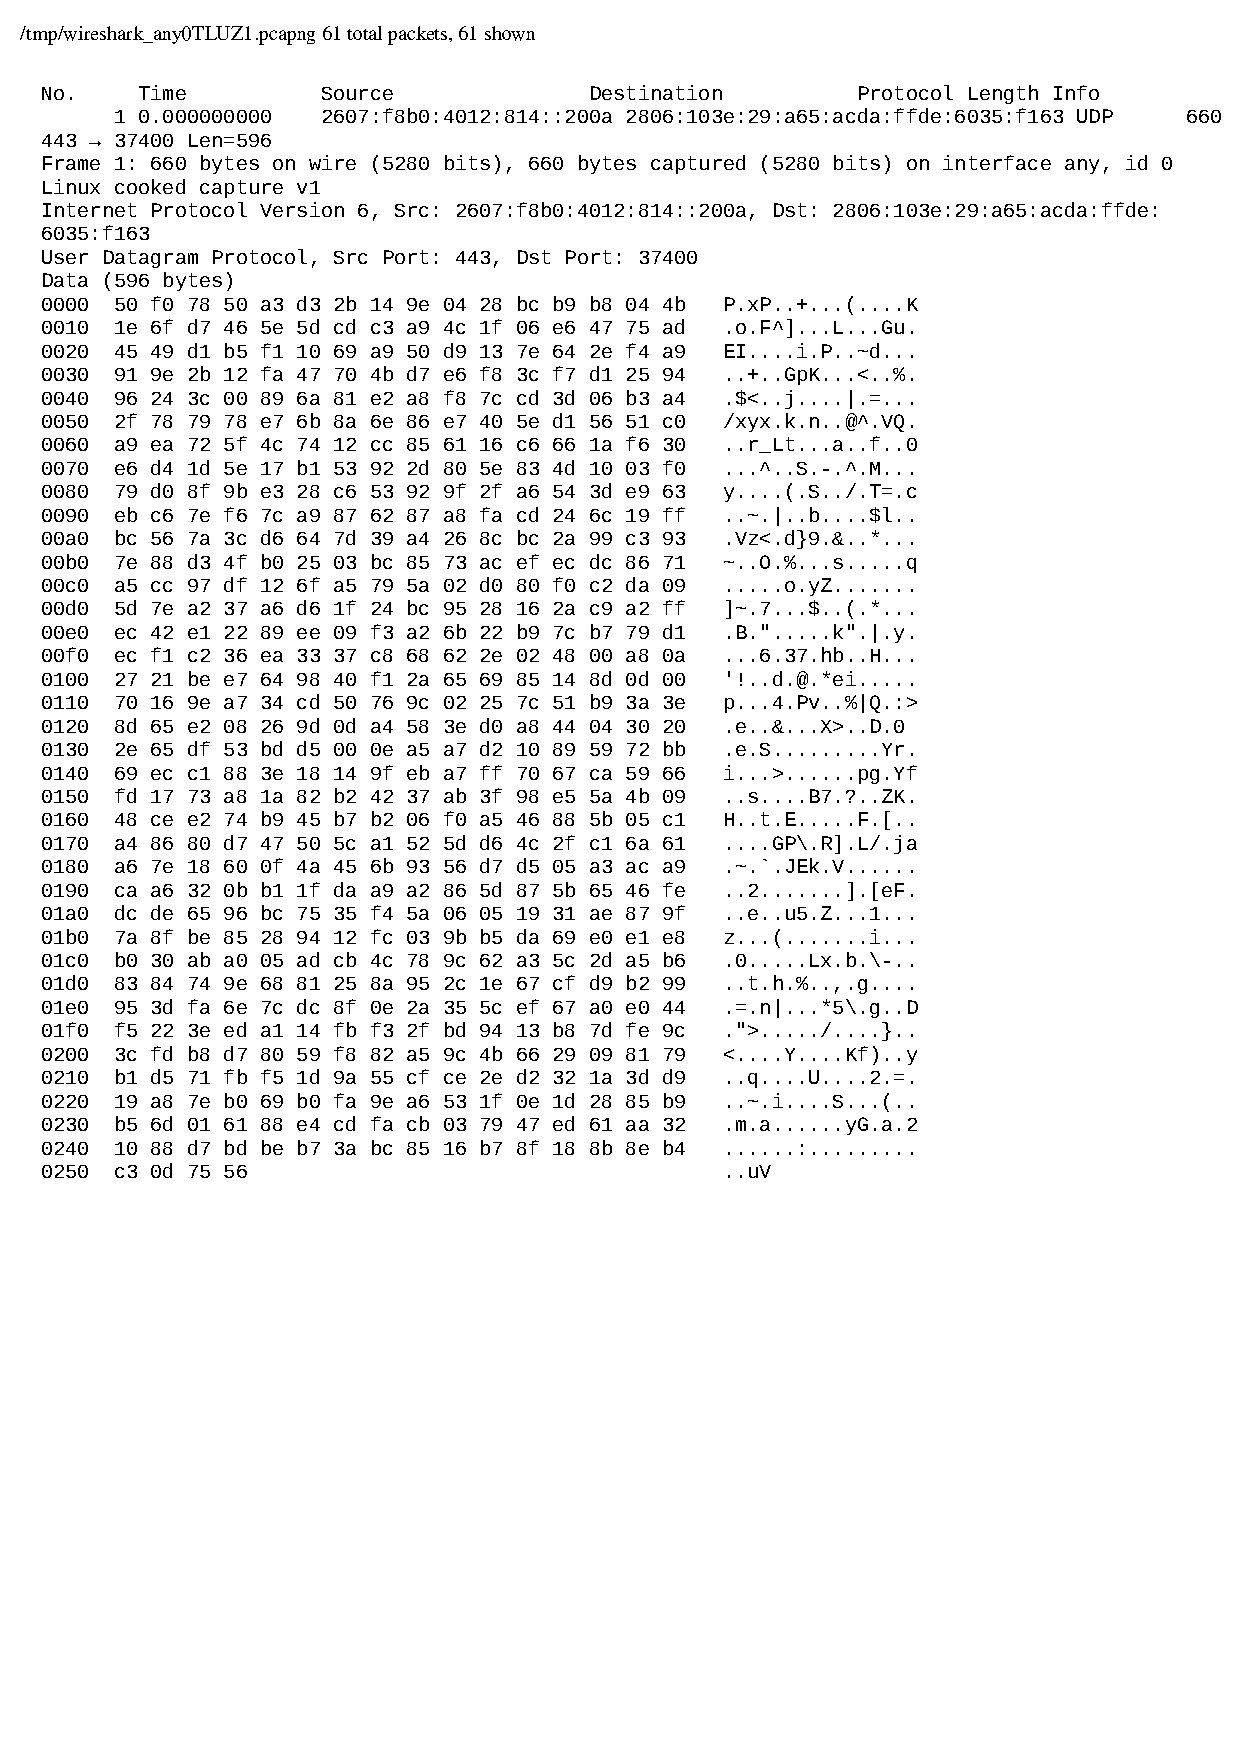
\includepdf[pages={1}]{/home/dieguito/Documents/3/AdminRedes/Reporte2/unpaquete.pdf}

La captura es muy extensa, pero desglosándolo todo se entiende un poco qué está pasando:

\begin{itemize}
	\item La primer dirección IP es una IP versión
	6, la cual está representada por 8 grupos de, generalmente cuatro carácteres hexadecimales, en este caso es la dirección
	IP corresponde a la de mi celular.
	\item La dirección de destino es también una
	dirección IPv6
\end{itemize}
La dirección destinatario apunta a\\

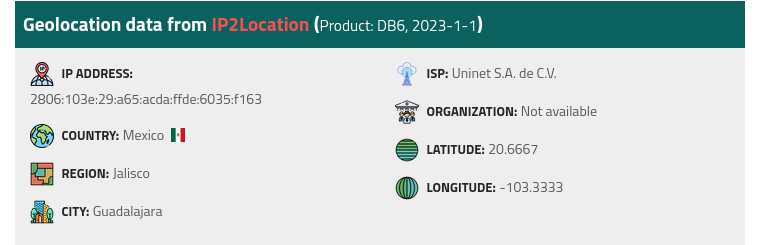
\includegraphics[scale=0.5]{/home/dieguito/Documents/3/AdminRedes/Reporte2/IP Address Lookup Geolocation.png}\\

Que parece ser la dirección del servidor de
Telmex en San Pedro Tlaquepaque\\

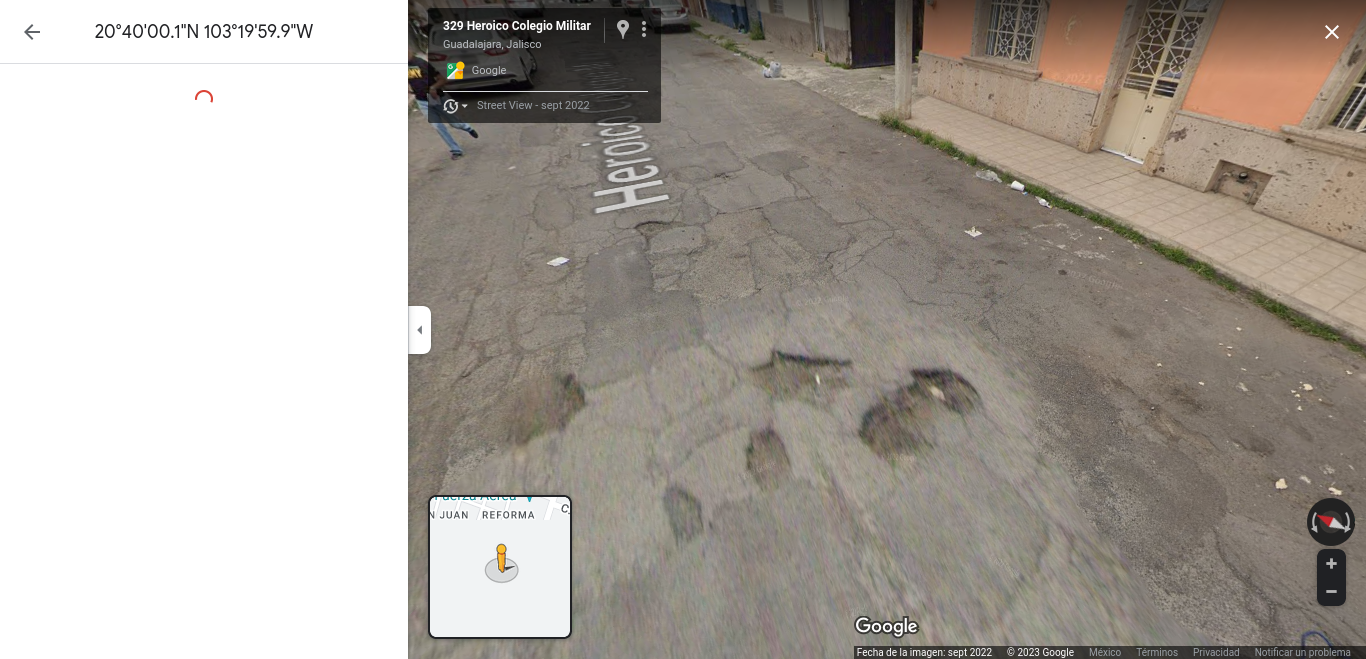
\includegraphics[scale=0.25]{/home/dieguito/Documents/3/AdminRedes/Reporte2/Google Maps.png}\\
Aunque en Google Maps muestre lo contrario.\\

Aún así, interesante.\\

El protocolo que utiliza la conexión es UDP, protocolo que especifica el puerto al cual quiere mandar la información.

Todo este tipo de información me es fascinante, aunque es mucha terminología de golpe, siento que con un poco de paciencia y dedicación, puedo entender por lo menos la mitad de lo que dice un mensaje en WireShark, que parece ser una herramienta muy útil para el hackeo ético.
\end{document}
